\chapter{Presentation of Results}
\section{Introduction}
The sections and subsections in this chapter describe the implementation, testing and results of the project. It starts by discussing how the web application to handle students' results was built. It then describes how The decentralised file storage element of the system was put up and how all these elements were integrated together.

\section{System Implementation}
This section and the subsections beneath it describe the Implementation and results of the project. Different elements of the system were built using different tools. The subsections below further describe how each element was built to get the complete system running from the web application that handles the students' results to the decentralised storage of transcripts and blockchain store for the hash values.

\subsection{Results System}
The results system is an element of the system where results are initially entered and processed before they are finally stored on a decentralised network. This system is built to be accessed by students, administrative assistants, the academic registrar and the system administrator. All these have different levels of priviledges when accessing the system for example, a student is only able to view his results and not edit them. The first attempt to build this system was done entirely on a blockchain network using smart contracts. 

\subsection{User Interface Design}
The system can be accessed through a web application on a browser of choice. However, the browser should be able to support the MetaMask file extension. This is helpful in enabling the user access the blockchain network.

\subsubsection{Account Creation}
For a student still on normal academic progress, he/she has the ability to register and have an account. This requires the student id number and a password. \\~\\
However, for access to the blockchain, the student or any other user intending to access the verified transcript has to create an account on the Ethereum\cite{art13} network. During this process, a seed phrase is automatically generated for a user and he/she only has to create a password.

\begin{figure}[!h]
\center
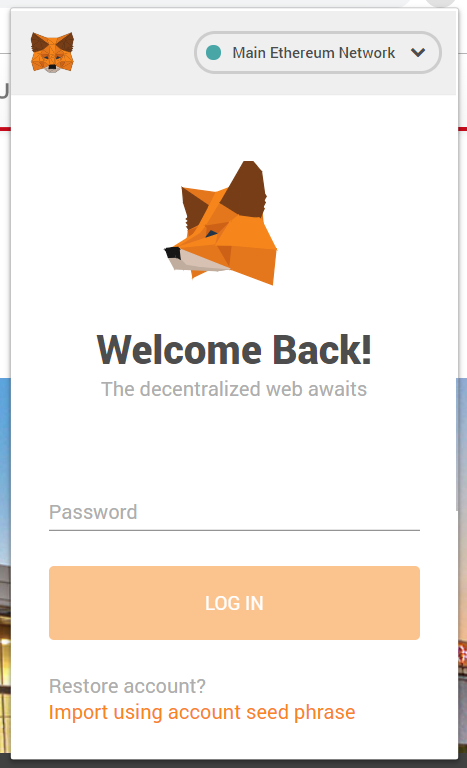
\includegraphics[scale=0.6]{images/metamasklogin.png}
\caption{Loging into the ethereum network}
\end{figure}

\subsubsection{Results}
\textbf{Viewing Results}\\~\\
This page can be accessed by a logged in student or an administrative assistant. The student can only view his/her results whereas the administrative assistant can view the results of various students.
\textbf{Manipulating results}\\~\\
In addtion to viewing results of various students, the adminsstrative assistant can also add/edit students’ results.
